\documentclass[hidelinks,aspectratio=169]{beamer}
\usepackage[italian]{babel} 
\usepackage[utf8]{inputenc} 
\usepackage{fourier} 


%Slide colors
\usetheme{Boadilla}
\usecolortheme{beaver}

% Images
\usepackage{graphicx}
\usepackage{caption}
\usepackage{subcaption}
\usepackage{float}
\graphicspath{ {../Images} }

% FlowChart
\usepackage{smartdiagram}

% Stop hyphenation
\usepackage[none]{hyphenat}

% Coloring links
\usepackage{xcolor}

% Enumerate abc
\usepackage{enumerate}

% Minipages in the same line
\usepackage{tabularx}

% Redefines caption setup in way to remove "Figure:"
\usepackage{caption}
\captionsetup[figure]{labelformat=empty}

% License
\usepackage[
type={CC},
modifier={by-nc-sa},
version={4.0},
]{doclicense}

% Command to enumerate frames title
\newcommand{\numcirc}[1]{%
	%   \usebeamerfont*{item projected}%
	\large
	\usebeamercolor[bg]{item projected}%
	\begin{pgfpicture}{-1ex}{0ex}{1ex}{2ex}
		\pgfpathcircle{\pgfpoint{0pt}{.75ex}}{1.2ex}
		\pgfusepath{fill}
		\pgftext[base]{\color{fg}#1}
	\end{pgfpicture}%
	\usebeamerfont*{frametitle}%
}

%Command to zoom in
\usepackage{mwe}
\makeatletter
\newsavebox\zb@x
\newcounter{z@@m}
\usepackage{calc}
\newdimen\B@r\newdimen\P@r
\newdimen\@zw\newdimen\@zh\newdimen\@zd

\newcommand{\zoombox}[2][0]{%
	\leavevmode%
	\sbox\zb@x{#2}%
	\setlength\B@r{1pt*\ratio{\wd\zb@x}{\ht\zb@x+\dp\zb@x}}%
	\setlength\P@r{1pt*\ratio{\paperwidth}{\paperheight}}%
	\ifdim\B@r>\P@r\relax%
	\setlength\@zw{\wd\zb@x}\setlength\@zh{\@zw*\ratio{\paperheight}{\paperwidth}}%
	\setlength\@zd{(\@zh-\ht\zb@x-\dp\zb@x)*\real{0.5}+\dp\zb@x}%
	\setlength\@zh{\@zh-\@zd}%
	\else%
	\setlength\@zh{\ht\zb@x+\dp\zb@x}%
	\setlength\@zw{\@zh*\ratio{\paperwidth}{\paperheight}}%
	\setlength\@zh{\ht\zb@x}\setlength\@zd{\dp\zb@x}%
	\fi%
	\makebox[0pt][l]{\makebox[\wd\zb@x][c]{\makebox[\@zw][l]{%
				\pdfdest name {zbfs\thez@@m} fitr
				width  \@zw\space
				height \@zh\space
				depth  \@zd\space
	}}}%
	\pdfdest name {zb\thez@@m} fitr
	width  \wd\zb@x\space
	height \ht\zb@x\space
	depth  \dp\zb@x\space
	\immediate\pdfannot 
	width  \wd\zb@x\space
	height \ht\zb@x\space
	depth  \dp\zb@x\space
	{%
		/Subtype/Link/H/N
		/Border [0 0 #1 [1 2]]
		/A <<
		/S/JavaScript
		/JS (
		if(typeof(zoomed)=='undefined'||!zoomed){
			var lastView=this.viewState;
			if(app.fs.isFullScreen) this.gotoNamedDest('zbfs\thez@@m');
			else this.gotoNamedDest('zb\thez@@m');
			zoomed=true;
		}else{
			this.viewState=lastView;
			zoomed=false;
		}
		)
		>>
	}%
	\usebox{\zb@x}%
	\stepcounter{z@@m}%
} 
\makeatother



%Header
\title[Identità e valore della stampa d'arte]{\textbf{Identità e valore della stampa d'arte}}
\author{Roberto Budassi}
\date{}

\begin{document}
	
		\begin{frame}
		\maketitle
		
		\vspace*{\fill}
		\centering
		\fboxrule=2pt
		\fbox
		{
			\begin{minipage}{0.9\linewidth}
				\small{Il seguente documento è ottimizzato per la visualizzazione digitale con \href{https://get.adobe.com/it/reader/}{\textcolor{blue}{Adobe~Acrobat~Reader}}.}  
			\end{minipage}
		}
	\end{frame}
	
	\begin{frame}
		\tableofcontents
	\end{frame}
	
	%--------------------- Include from here  -----------------
	
	\section{Tiratura, segnatura e numerazione}
	\begin{frame}{Tiratura, segnatura e numerazione}
		\begin{itemize}
			\item Bon a Tirer
			\item Tiratura corrente: non numerata e non firmata – a forte tiratura (acciaiatura)
			\item Numerazione araba: 1/100 – 100/100
			\item Numerazione romana: I/XV – XV/XV
			\item Alfabetica: a, b, c, d, … etc. etc
			\item Prova d’artista - prova d’autore - épreuve d’artiste - artist’s proof: P.A., P.d.A., E.A., A.P. 
			\item Fuori Commercio - Hors Commerce: F.C. H.C.
			\item Prova di Stampa: P.d.S.; E.E.
			\item Prova colore: P.C., P.d.C.
			\item Tiratura dopo la biffatura (cancellazione) del rame
		\end{itemize}
		\medskip
		\begin{itemize}
			\item Tiratura coeva
			\item Tiratura postuma
			\item Tiratura tarda
			\item Tiratura moderna
		\end{itemize}
	\end{frame}
	
	\begin{frame}{Tiratura, segnatura e numerazione}
		\begin{tabularx}{\linewidth}{XXX}
			{
			\centering
			\zoombox{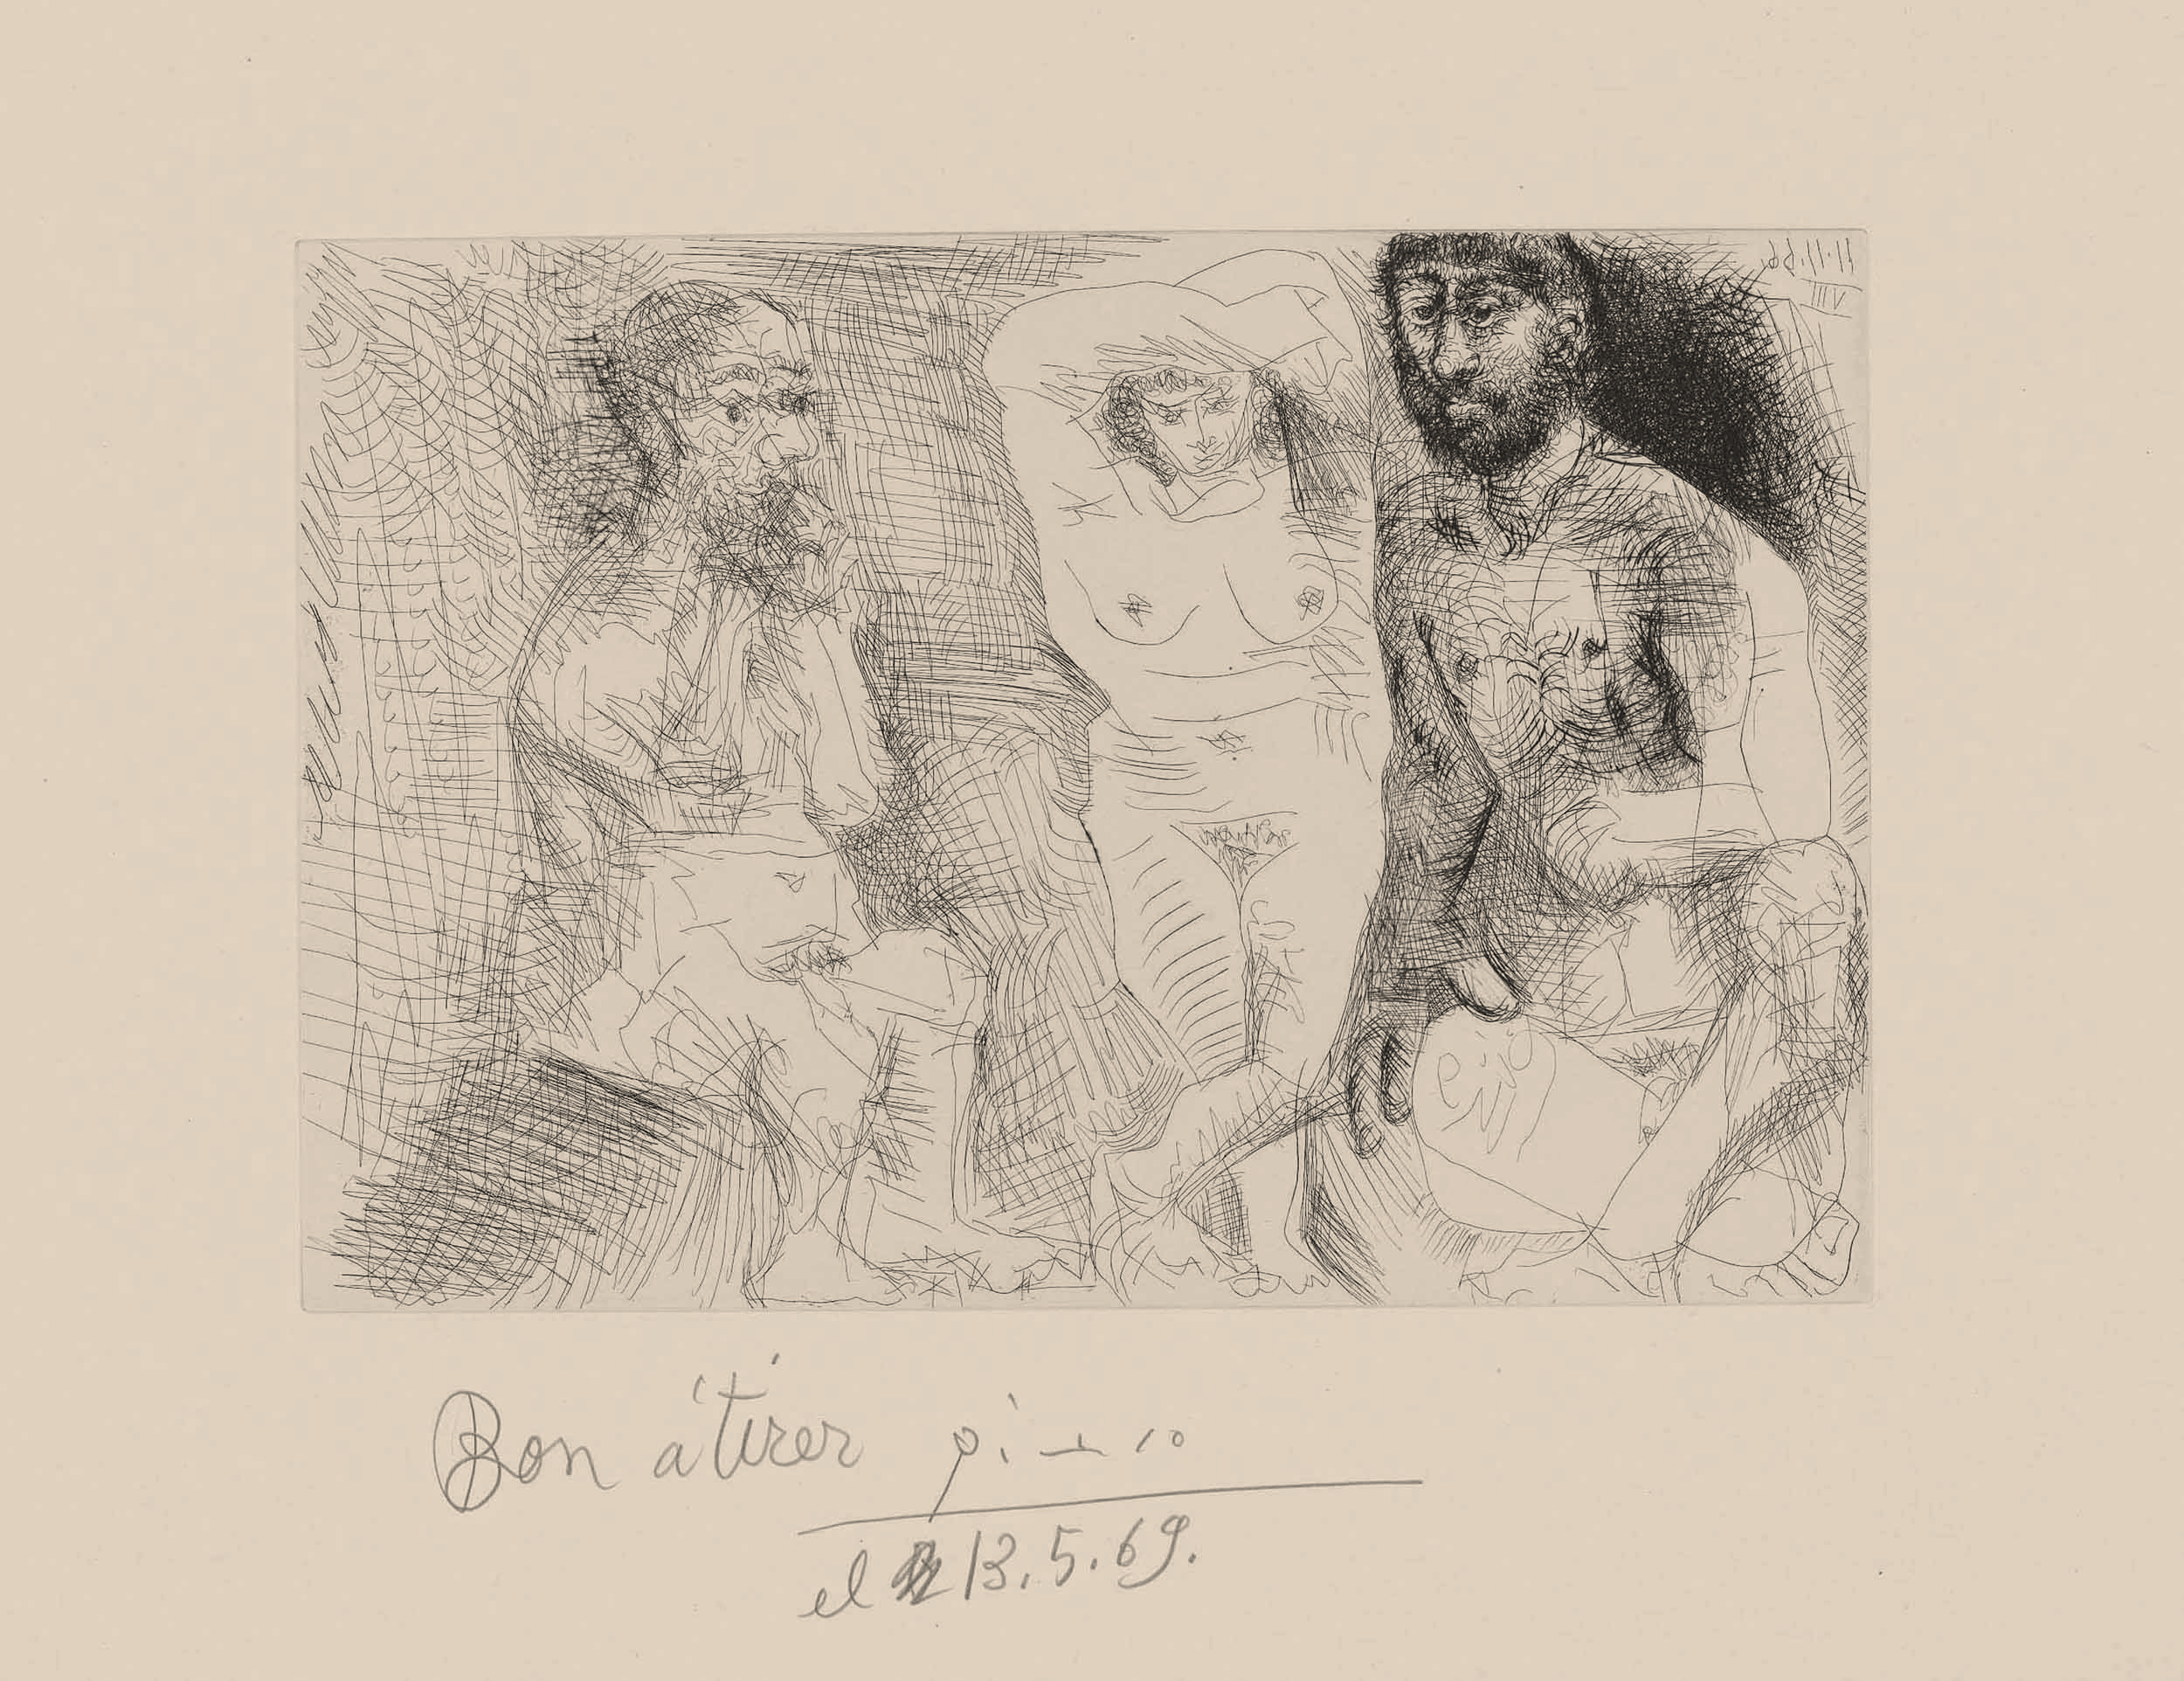
\includegraphics[scale=0.09]{Pablo Picasso, soggetti dalla serie 374-1.png}}
			}&{
			\centering
			\hspace*{1.7mm}
			\zoombox{\includegraphics[scale=0.2]{Pablo Picasso, soggetti dalla serie 374-2.png}}
			}&{
			\centering
			\zoombox{\includegraphics[scale=0.205]{Pablo Picasso, soggetti dalla serie 374-3.png}}
			}
		\end{tabularx}
		\centering
		\small{Pablo Picasso, soggetti dalla serie 374, esemplari di Bon a tirer, Prova d’artista e in numerazione araba}
	\end{frame}
	
	\subsection{Il remarque}
	\begin{frame}{Il remarque}
		\begin{tabularx}{\linewidth}{XX}
			{
			\centering
			\hspace*{19mm}
			\zoombox{\includegraphics[scale=0.4]{Pablo Picasso, frammento di corpo1.jpg}}
			}&{
			\centering
			\hspace*{9mm}
			\zoombox{\includegraphics[scale=0.41]{Pablo Picasso, frammento di corpo2.jpg}}
			}
		\end{tabularx}
		\centering
		\small{Pablo Picasso, frammento di corpo, da Le metamorfosi di Ovidio, acquaforte}
	\end{frame}
	
	\subsection{La biffatura}
	\begin{frame}{La biffatura}
		\begin{tabularx}{\linewidth}{XXX}
			{
			\centering
			%\hspace*{19mm}
			\zoombox{\includegraphics[scale=0.4]{Pablo Picasso, frammento di corpo1.jpg}}
			}&{
			\centering
			%\hspace*{9mm}
			\zoombox{\includegraphics[scale=0.41]{Pablo Picasso, frammento di corpo2.jpg}}
			}&{
			\centering
			%\hspace*{9mm}
			\zoombox{\includegraphics[scale=0.51]{Pablo Picasso, frammento di corpo3.png}}
			}
		\end{tabularx}
		\centering
		\small{Pablo Picasso, frammento di corpo, da Le metamorfosi di Ovidio, acquaforte}
	\end{frame}
	
	\begin{frame}{La biffatura}
		\begin{tabularx}{\linewidth}{XX}
			{
			\centering
			\hspace*{8mm}
			\zoombox{\includegraphics[scale=0.7]{Edgar Degas1.png}}
			}&{
			\centering
			\hspace*{8mm}
			\zoombox{\includegraphics[scale=0.24]{Edgar Degas2.png}}
			}
		\end{tabularx}
		\centering
		\small{Edgar Degas, Le stiratrici, acquaforte e acquatinta}
	\end{frame}
	
	\subsection{La rarità}
	\begin{frame}{La rarità}
		\begin{tabularx}{\linewidth}{XX}
			{
				\vspace*{-5mm}
			\small{Rarità (riguarda la quantità di esemplari)}
			\begin{itemize}
				\item[] 
				\begin{itemize}
					\item \footnotesize{Unico}
					\item \footnotesize{Rarissimo}
					\item \footnotesize{Raro}
					\item \footnotesize{Comune}
				\end{itemize}
				
			\end{itemize}
			%\bigskip
			\small{Qualità (riguarda la bellezza dell'impressione)}
			\begin{itemize}
				\item \footnotesize{Stampe moderne}
				\vspace*{-1mm}
				\begin{itemize}
					\item \footnotesize{Perfetto esemplare}
				\end{itemize}
				\item \footnotesize{Stampe antiche}
				\vspace*{-1mm}
				\begin{itemize}
					\item \footnotesize{Splendida}
					\item \footnotesize{Magnifica}
					\item \footnotesize{Bellissima}
					\item \footnotesize{Bella}
					\item \footnotesize{Discreta}
					\item \footnotesize{Mediocre}
					\item \footnotesize{Stanca}
					\item \footnotesize{Povera}
				\end{itemize}
			\end{itemize}
			}&{
			\vspace*{15mm}
			\begin{tabularx}{\linewidth}{XX}
				{
				\centering
				\zoombox{\includegraphics[scale=0.21]{Paul Gauguin1.jpg}}
				}&{
				\centering
				\zoombox{\includegraphics[scale=0.2]{Paul Gauguin2.png}}
				}
			\end{tabularx}
			\centering
			\small{Paul Gauguin, La mercante di fichi, acquaforte e acquatinta}
			}
		\end{tabularx}
	\end{frame}
	
	\begin{frame}{La rarità}
		\begin{tabularx}{\linewidth}{XX}
			{
			\centering
			\hspace*{15mm}
			\zoombox{\includegraphics[scale=0.07]{Rembrandt9.jpg}}
			}&{
			\centering
			\hspace*{15mm}
			\zoombox{\includegraphics[scale=0.4]{Rembrandt10.jpg}}
			}
		\end{tabularx}
		\centering
		\small{Rembrandt, Cristo che guarisce gli ammalati o stampa dei cento fiorini, acquaforte, acquatinta e puntasecca - Pablo Picasso, Il pasto frugale, acquaforte}
	\end{frame}
	
	\begin{frame}{La rarità}
		\begin{tabularx}{\linewidth}{XX}
			{
			\centering
			\hspace*{15mm}
			\zoombox{\includegraphics[scale=0.25]{Vincent Van Gogh1.jpg}}
			}&{
			\centering
			\hspace*{15mm}
			\zoombox{\includegraphics[scale=0.51]{Vincent Van Gogh2.jpg}}
			}
		\end{tabularx}
		\centering
		\small{Vincent Van Gogh, I mangiatori di patate, litografia - Ritratto del Dottor Gachet, acquaforte}
	\end{frame}
	
	\begin{frame}{La rarità}
		\begin{tabularx}{\linewidth}{XX}
			{
			\centering
			\hspace*{11mm}
			\zoombox{\includegraphics[scale=0.7]{Rembrandt11.jpg}}
			}&{
			\centering
			\hspace*{11mm}
			\zoombox{\includegraphics[scale=0.37]{Rembrandt12.jpg}}
			}
		\end{tabularx}
		\centering
		\small{Rembrandt, La morte della Vergine Maria, acquaforte e puntasecca nelle prima tiratura e in tiratura moderna}
	\end{frame}
	
	\subsection{Misure e Margini}
	\begin{frame}{Misure e Margini}
		\centering \textbf{Misure}
		\begin{tabularx}{\linewidth}{XX}
			{
				\vspace*{-35mm}
				\begin{itemize}
					\item \footnotesize{\textbf{Matrice}\\ Altezza per larghezza, in millimetri, rilevate:}
					\begin{itemize}
						\item \footnotesize{All'impronta del rame}
						\item \footnotesize{Ai margini dell'impressione xilografica}
						\item \footnotesize{Ai limiti del disegno litografico}
					\end{itemize}
					\item \footnotesize{\textbf{Foglio}\\ Altezza per larghezza, in centimetri}
				\end{itemize}
			}&{
			\centering
			\hspace*{15mm}
			\zoombox{\includegraphics[scale=0.6]{Marc Chagall1.jpg}}
			}
		\end{tabularx}
		\centering \textbf{Margini}
		\begin{tabularx}{\linewidth}{XX}
			{
				\vspace*{-35mm}
				\begin{itemize}
					\item \footnotesize{Tagliati all’interno dell’impronta}
					\item \footnotesize{Tagliati all’impronta del rame}
					\item \footnotesize{Editoriali (senza margini)}
					\item \footnotesize{Tagliati oltre l’impronta de rame per mm…}
					\item \footnotesize{Intonsi (misure del foglio)}
					\item \footnotesize{Rimarginato (ricostruito)}
				\end{itemize}
				\begin{minipage}{\linewidth}
						\tiny{Marc Chagall, Il bouquet di fiori, litografia a colori in tiratura de luxe con grandi margini e in tiratura corrente con margini editoriali}
				\end{minipage}
			}&{
			\centering
			\hspace*{15mm}
			\zoombox{\includegraphics[scale=0.27]{Marc Chagall2.png}}
			}
		\end{tabularx}
	\end{frame}
	
	\subsection{Autenticità e datazione}
	\begin{frame}{\textbf{Autenticità e datazione}\\ Il supporto: carta e filigrana}
		\begin{tabularx}{\linewidth}{XX}
			{
			\centering
			\hspace*{8mm}
			\zoombox{\includegraphics[scale=0.4]{Carta1.png}}
			}&{
			\centering
			\hspace*{8mm}
			\zoombox{\includegraphics[scale=0.15]{Carta2.png}}
			}
		\end{tabularx}
	\end{frame}
	
	\subsection{Monogrammi - Firma - Timbri}
	\begin{frame}{Monogrammi - Firma - Timbri}
		\begin{tabularx}{\linewidth}{XX}
			{
			\centering
			\hspace*{8mm}
			\zoombox{\includegraphics[scale=0.4]{Monogramma1.jpg}}
			}&{
			\vspace*{-40mm}
			Inscrizioni di attribuzione e responsabilità
			\begin{itemize}
				\item \footnotesize{Inv.., invenit, inventor: inventore del soggetto}
				\item \footnotesize{p. pin., pinxit: chi dipinse il soggetto}
				\item \footnotesize{del. – delin.: delineavit: disegnatore del soggetto}
				\item \footnotesize{Exc. Excudit: stampatore}
				\item \footnotesize{f., faciebat, fec., fecit: incisore del soggetto}
				\item \footnotesize{Scalp., scalpsit, sculp., Sculpsit: incise }
			\end{itemize}
			}
		\end{tabularx}
		\vspace*{3mm}
		\centering
		\zoombox{\includegraphics[scale=0.25]{Monogramma2.png}}
	\end{frame}
	
	\begin{frame}{Monogrammi - Firma - Timbri}
		\begin{tabularx}{\linewidth}{XXX}
			{
			\centering
			\zoombox{\includegraphics[scale=0.2]{Firma1.jpg}}
			}&{
			\centering
			\hspace*{10mm}
			\zoombox{\includegraphics[scale=0.4]{Firma2.jpg}}
			}&{
			\centering
			\hspace*{-15mm}
			\zoombox{\includegraphics[scale=0.55]{Firma3.jpg}}
			}
		\end{tabularx}
	\end{frame}
	
	\subsection{Firma - Sigle - Timbri}
	\begin{frame}{Firma - Sigle - Timbri}
		\begin{tabularx}{\linewidth}{XXX}
			{
			\centering
			%\vspace*{1mm}
			\zoombox{\includegraphics[scale=0.22]{Sigla1.jpg}}
			}&{
			\centering
			\vspace*{-50mm}
			\zoombox{\includegraphics[scale=0.2]{Sigla2.png}}
			\newline
			\medskip
			\zoombox{\includegraphics[scale=0.25]{Sigla3.png}}
			\newline
			\medskip
			\zoombox{\includegraphics[scale=0.3]{Sigla4.png}}
			}&{
			\centering
			\hspace*{-5mm}
			\zoombox{\includegraphics[scale=0.35]{Sigla5.png}}
			}
		\end{tabularx}
	\end{frame}
	
	\begin{frame}{Firma - Sigle - Timbri}
		\begin{tabularx}{\linewidth}{X}
			{
			\begin{center}
				\vspace*{-5mm}
				\zoombox{\includegraphics[scale=0.2]{Sigla6.png}}
			\end{center}
			}
		\end{tabularx}
	\end{frame}
	
	\begin{frame}{Firma e/o Filigrana}
		\begin{tabularx}{\linewidth}{XXX}
			{
			\centering
			\zoombox{\includegraphics[scale=0.4]{Filigrana1.png}}
			}&{
			\centering
			\zoombox{\includegraphics[scale=0.25]{Filigrana2.png}}
			}&{
			\centering
			\zoombox{\includegraphics[scale=0.2]{Filigrana3.png}}
			}
		\end{tabularx}
		\begin{tabularx}{\linewidth}{XXX}
			{
			\centering
			\zoombox{\includegraphics[scale=0.3]{Filigrana4.png}}
			}&{
			\centering
			\zoombox{\includegraphics[scale=0.25]{Filigrana5.png}}
			}&{
			\centering
			\zoombox{\includegraphics[scale=0.15]{Filigrana6.png}}
			}
		\end{tabularx}
	\end{frame}
	
	\subsection{Restauro - Conservazione - Documentazione - Fruizione}
	\begin{frame}{Restauro - Conservazione - Documentazione - Fruizione}
		\begin{tabularx}{\linewidth}{XX}
			{
			\centering
			\textbf{Stato di conservazione} (riguarda il supporto cartaceo)
			\begin{itemize}
				\item  \small{Eccezionale}
				\item  \small{Perfetto}
				\item  \small{Buono}
				\item  \small{Difettoso}
				\item  \small{Cattivo}
			\end{itemize}
			}&{
			\centering
			\textbf{Difetti}
			\begin{itemize}
				\item \small{Incollata}
				\item \small{Riparata}
				\item \small{Danneggiata}
				\item \small{Graffi e/o Raschiature}
				\item \small{Lacerata e/o Strappata}
				\item \small{Macchie d’umido – Foxes}
				\item \small{Polvere e/o Sporco}
				\item \small{Parti mancanti}
				\item \small{Pieghe}
			\end{itemize}
			}
		\end{tabularx}
	\end{frame}
	
	\begin{frame}{Restauro - Conservazione - Documentazione - Fruizione}
		\begin{tabularx}{\linewidth}{XX}
			{
			\centering
			\hspace*{7mm}
			\zoombox{\includegraphics[scale=0.42]{Conservazione1.png}}
			}&{
			\centering
			\hspace*{7mm}
			\zoombox{\includegraphics[scale=0.37]{Conservazione2.png}}
			}
		\end{tabularx}
	\end{frame}
	
	\begin{frame}{Restauro - Conservazione - Documentazione - Fruizione}
		\begin{tabularx}{\linewidth}{XX}
			{
			\centering
			\hspace*{15mm}
			\zoombox{\includegraphics[scale=0.35]{Conservazione3.jpg}}	
			}&{
			\centering
			\hspace*{-5mm}
			\zoombox{\includegraphics[scale=0.4]{Conservazione4.jpg}}
			}
		\end{tabularx}
	\end{frame}
	
	\begin{frame}{Restauro - Conservazione - Documentazione - Fruizione}
		\begin{tabularx}{\linewidth}{X}
			{
			\begin{center}
				\vspace*{-8mm}
				\zoombox{\includegraphics[scale=0.33]{Conservazione5.png}}
			\end{center}
			}
		\end{tabularx}
	\end{frame}
	
	\begin{frame}{Restauro - Conservazione - Documentazione - Fruizione}
		\begin{tabularx}{\linewidth}{XX}
			{
			\centering
			\hspace*{15mm}
			\zoombox{\includegraphics[scale=0.4]{Braque1.png}}
			}&{
			\vspace*{-65mm}
			\textbf{Braque Georges}
			\newline
			(Argenteuil 1882 - Parigi 1963)
			\newline
			\hrule
			\bigskip
			\small{\textit{Vaso}, 1950, I/I \newline
			(Dora Vallier 59, E. 35, BN. 43, M. 19)\newline
			Acquaforte, inciso mm. 240 x 105, foglio Arches RFK Rives, esemplare numerato 8/10; sul foglio, a matita, firma; edizione di 40 di cui 10 su India cm. 40 x 24, 10 su Giappone imperiale cm. 50 x 32, 10 su Chiffon cm. 38 x 20, 10 su Arches RFK Rives, più alcune prove d’artista. Stampatore Signovert di Parigi su torchio di Braque; editore A. Maeght – Parigi; lastra in possesso dell’artista. \newline
			inv. C.IV.84. 112 (4000 P.Prouté – Parigi)}
			}
		\end{tabularx}
	\end{frame}
	
	\subsection{Libri consigliati}
	\begin{frame}{Libri consigliati}
		\begin{tabularx}{\linewidth}{XXXX}
			{
			\centering
			\zoombox{\includegraphics[scale=0.07]{Libro1.png}}
			}&{
			\centering
			\zoombox{\includegraphics[scale=0.3]{Libro2.png}}
			}&{
			\centering
			\zoombox{\includegraphics[scale=0.16]{Libro3.png}}
			}&{
			\centering
			\zoombox{\includegraphics[scale=0.3]{Libro4.png}}
			}
		\end{tabularx}
		\begin{tabularx}{\linewidth}{XXXX}
			{
			\centering
			\zoombox{\includegraphics[scale=0.115]{Libro5.png}}	
			}&{
			\centering
			\zoombox{\includegraphics[scale=0.06]{Libro6.jpg}}
			}&{
			\centering
			\zoombox{\includegraphics[scale=0.08]{Libro7.png}}
			}&{
			\centering
			\zoombox{\includegraphics[scale=0.055]{Libro8.jpg}}
			}
		\end{tabularx}
		\begin{tabularx}{\linewidth}{XXXXXXX}
			{
			\centering
			\zoombox{\includegraphics[scale=0.1]{Libro9.png}}
			}&{
			\centering
			\zoombox{\includegraphics[scale=0.22]{Libro10.jpg}}
			}&{
			\centering
			\zoombox{\includegraphics[scale=0.1]{Libro11.jpg}}
			}&{
			\centering
			\zoombox{\includegraphics[scale=0.1]{Libro12.jpg}}
			}&{
			\centering
			\zoombox{\includegraphics[scale=0.1]{Libro13.jpg}}
			}&{
			\centering
			\zoombox{\includegraphics[scale=0.1]{Libro14.jpg}}
			}&{
			\centering
			\zoombox{\includegraphics[scale=0.05]{Libro15.jpg}}
			}
		\end{tabularx}
	\end{frame}
	
	\begin{frame}{Libri consigliati}
		\begin{itemize}
			\item \tiny{Gariazzo P.A., La stampa incisa, Lattes, Torino 1907}
			\item \tiny{Pittaluga M. L’incisione italiana del cinquecento, Hoepli, Milano 1928}
			\item \tiny{Bosse A., Bosse e il suo trattato della calcografia, Cesare Ratta Ed., Bologna 1937}
			\item \tiny{De Witt A., Incisione italiana, Ed. U. Hoepli, Milano 1950}
			\item \tiny{Mallè G., L’incisione europea dal XV al XX secolo, Galleria Civica d’Arte Moderna, Torino 1968}
			\item \tiny{Salamon F., La collezione di stampe, Mondadori, Milano 1971}
			\item \tiny{Tedeschi N., La stampa degli artisti, Fiorini, Verona 1971}
			\item \tiny{Strazza G. Il gesto e il segno, Scheiwiller, Milano 1979}
			\item \tiny{Battistoni A., Tecniche dell’incisione, Quattro Venti, Urbino 1983}
			\item \tiny{Bianchi Barriviera L., L’incisione e la stampa originale. Tecniche antiche e moderne, Neri Pozza, Vicenza 1984}
			\item \tiny{Federici R., Kraczyna S., Viggino D., I segni incisi. Guida alla xilografia e all’incisione, Il Bisonte, Firenze 1985}
			\item \tiny{Paglialonga B., La calcografia, Riccitelli, Pescara 1985}
			\item \tiny{Massari S., Negri Arnoldi F., Arte e scienza dell’incisone. Da Maso Finiguerra a Picasso, Carocci, Roma 1987}
			\item \tiny{Bruscaglia R., Incisione calcografica e stampa originale d’arte. Materiali, procedimenti, segni grafici. Quattroventi, Urbino 1988}
			\item \tiny{Mariani G., Acquaforte Acquatinta Lavis Ceramolle. Le tecniche calcografiche d’incisione indiretta, Istituto Nazionale Per La Grafica, De Luca Editori D’Arte, Roma 2005}
			\item \tiny{Esposito Hayter C. Il monotipo. Storia di un’arte pittorica. Skira, Milano 2007}
			\item \tiny{De Stefano M., Guida Pratica alle tecniche di incisione. Procedimenti della calcografia tradizionale moderna-sperimentale e atossica. Prinp Editore, Torino 2016}
		\end{itemize}
		
		\begin{itemize}
			\item \tiny{Benjamin W., “L’opera d’arte nell’epoca della sua riproducibilità tecnica”, Einaudi, Torino 1966}
			\item \tiny{Petrucci C.A., voce “Incisione” in Enciclopedia Universale dell’Arte, vol. VIII, Venezia- Roma 1968}
			\item \tiny{Kandinsky V., “Punto, linea, superficie”, Adelphi, Milano 1968}
			\item \tiny{Giubbini G., Parma Armani E., “Incisione e stampa” in Le Tecniche artistiche, Mursia, Milano 1973}
		\end{itemize}
	\end{frame}
	
\end{document}